\documentclass[a4paper,11pt,fleqn]{article}%fleqn pour aligner les equations à gauche

\usepackage{../../Styles/Cours}

\newcommand{\chnum}{Chapitre 7}
\newcommand{\chtitle}{Équilibres acide-base}
\newcommand{\dtype}{Cours}


\begin{document}
\maketitle

\section{Réaction d'un acide ou d'une base avec l'eau}
L'eau est une espèce amphotère (couples \ce{H3O+(aq)} / \ce{H2O(l)} et \ce{H2O(l)}/\ce{HO-(aq)}). De ce fait, un acide peut réagir avec la base \ce{H2O} (premier couple) et une base peut réagir avec l'acide \ce{H2O} (deuxième couple).
	\subsection{Acides et bases fortes}
	Lorsque la réaction d'un acide avec l'eau est quasi-totale, l'acide est dit fort.\\
	L'équation s'écrit alors avec une simple flèche : \ce{AH(aq) + H2O(l) -> A-(aq) + H3O+(aq)}\\
	Lorsque la réaction d'une base avec l'eau est quasi-totale, la base est dite forte.\\
	L'équation s'écrit alors avec une simple flèche : \ce{A-(aq) + H2O(l) -> AH(aq) + HO-(aq)}
	\subsection{Acides et bases faibles}
	Lorsque la réaction d'un acide avec l'eau est non totale, l'acide est dit faible.\\
	L'équation s'écrit alors avec une double flèche : \ce{AH(aq) + H2O(l) <=> A-(aq) + H3O+(aq)}\\
	Lorsque la réaction d'une base avec l'eau est non totale, la base est dite faible.\\
	L'équation s'écrit alors avec une double flèche : \ce{A-(aq) + H2O(l) <=> AH(aq) + HO-(aq)}
	\subsection{Solutions courantes d'acide et de bases}
	\begin{tabular}{|>{\centering}m{9cm}|>{\centering\arraybackslash}m{9cm}|}
	\hline \textbf{Solutions d'acides forts} & \textbf{Solutions de bases fortes}\\
	\hline Acide chlorhydrique (\ce{H3O+(aq), Cl-(aq)}) & \multirow{2}{9cm}{Hydroxyde de sodium (soude) (\ce{Na+(aq), HO-(aq)})}\\
	Acide nitrique (\ce{H3O+(aq), NO3-(aq)}) & \\
	\hline \textbf{Solutions d'acides faibles} & \textbf{Solutions de bases faibles}\\
	\hline Acide éthanoïque \ce{CH3COOH(aq)} & Ammoniac \ce{NH3(aq)}\\
	\hline
	\end{tabular}
\section{Force des acides et des bases}
	\subsection{Constante d'acidité}
	Lors de la réaction d'un acide faible avec l'eau, le système chimique atteint un état d'équilibre. La constant d'équilibre de cette réaction est appelée \textbf{constante d'acidité} et notée $K_A$. Elle est caractéristique d'un couple acide base \ce{AH(aq)/A-(aq)}.\\
	Pour la réaction d'équation \ce{AH(aq) + H2O(l) <=> A-(aq) + H3O+(aq)}, on a :
	$$K_A = Q_{r,\text{éq}} = \dfrac{\dfrac{[\ce{A-(aq)}]_{\text{éq}}}{c^0} \times \dfrac{[\ce{H3O+}]_{\text{éq}}}{c^0}}{\dfrac{[\ce{AH}]_{\text{éq}}}{c^0}} = \dfrac{[\ce{A-(aq)}]_\text{éq} \times [\ce{H3O+}]_{\text{éq}}}{[\ce{AH}]_{\text{éq}} \times c^0} \nonumber$$
	avec $c^0 = \SI{1}{\mole \per \liter}$\\
	On définit aussi le $pK_A$ :
	$$pK_A = - \log{K_A} \leftrightarrow K_A = 10^{-pK_A}$$
	La constante d'acidité $K_A$ et le $pK_A$ permettent de comparer la force des acides et des bases faibles : \\
	Plus le $pK_A$ d'un couple est petit, plus sa constante d'acidité est grande, donc plus l'acide se dissocie dans l'eau et donc plus il est fort.
	\subsection{Produit ionique de l'eau}
	L'eau appartient à deux couples acide-base \ce{H3O+(aq)} / \ce{H2O(l)} et \ce{H2O(l)}/\ce{HO-(aq)}. Il peut donc se produire une réaction nommée \textbf{autoprotolyse de l'eau} entre la base \ce{H2O(l)} et l'acide \ce{H2O(l)} :
$$\ce{H2O(l) + H2O(l) <=> H3O+(aq) + HO-(aq)}$$
c'est à dire : $ \ce{2 H2O(l)}\ce{<=> H3O+(aq) + HO-(aq)}$\\
La constante d'équilibre associée à l'autoprotolyse de l'eau est appelée \textbf{produit ionique de l'eau} et est notée $K_e$. On aura :
$$K_e = \dfrac{\dfrac{[\ce{HO-(aq)}]_{\text{éq}}}{c^0} \times \dfrac{[\ce{H3O+}]_{\text{éq}}}{c^0}}{1} = \dfrac{[\ce{HO-(aq)}]_{\text{éq}} \times [\ce{H3O+}]_{\text{éq}}}{(c^0)^2}$$
Comme pour une constante d'acidité, il est courant d'utiliser $pK_e = -\log{K_e} \leftrightarrow K_e = 10^{-pK_e}$.\\
À \num{25} \unit{\celsius}, $K_e$ = \num{1,0e-14} et $pK_e = 14$

\section{Espèce prédominante d'un couple}
	\subsection{Diagramme de distribution et de prédominance}
	Une solution aqueuse à l'équilibre contient l'acide \ce{AH} d'un couple et la base \ce{A-} d'une solution en fonction de son pH à l'aide d'un \textbf{diagramme de distribution}.\\
	\begin{center}
	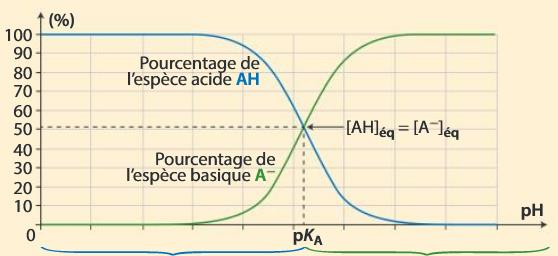
\includegraphics[scale=.7]{Ressources/TSPE_C8_Cours_Fig1.png}
	\end{center}
	Le diagramme de distribution précédent peut être simplifié en un \textbf{diagramme de prédominance} décrivant l'espèce majoritaire en fonction de la valeur du pH de la solution.\\
	
	\begin{center}
	\begin{tikzpicture}
\node (O) at (0,0) {};
\node (A) at (6,0) {};
\node (B) at (12,0) {};
\node (F) at (13,0) {};
\node (PredUp) at (3,.5) {$[AH]_{\text{éq}} > [A-]_{\text{éq}}$};
\node (PredDwn) at (3,-.5) {\textbf{\ce{AH} prédomine}};
\node (DomUp) at (9,.5) {$[AH]_{\text{éq}} < [A-]_{\text{éq}}$};
\node (DomDwn) at (9,-.5) {\textbf{\ce{A-} prédomine}};
\draw (O) node{$|$} node[below]{0};
\draw (A) node{$|$} node[below]{$pK_A$};
\draw (B) node{$|$} node[below]{14};
\draw[->] (O) to (F);
%\draw[->,>=latex] (L) to[bend left] (S);
%\draw[->,>=latex] (S) to[bend left] (P);
\end{tikzpicture}
\end{center}
	\subsection{Solutions tampons}
	\textbf{Une solution tampon est une solution dont le pH varie très peu lorsqu'on la dilue ou lorsqu'on y ajoute de petites quantités d'acide ou de base.} Elle contient un acide faible et sa base conjuguée en concentrations de même ordre de grandeur. Le pH d'une telle solution est donc proche du $pK_A$ du couple acide-base présent dans la solution.\\
	Exemple : 
	\begin{itemize}
		\item Les solutions utilisées pour étalonner les pH-mètres sont des solutions tampons.
		\item Le sang est un milieu tamponné. Son pH garde une valeur comprise entre 7,35 et 7,45, même lorsque nous faisons de l'exercice et que nos muscles produisent de l'acide lactique.
	\end{itemize}
	\subsection{Acides alpha-aminés}
	\begin{tabular}{m{4cm} m{14cm}}
	\chemfig{R-CH(-[:90]NH_2)-CO_2H} & Un \textbf{acide alpha-aminé} est une molécule qui contient un \textbf{groupe carbonyle \ce{-CO2H}} et un groupe \textbf{amine \ce{-NH2}} portés par le même atome de carbone.\\
	\end{tabular}\\
	Les acides alpha-aminés sont des espèces \textbf{amphotères} qui possèdent des propriétés acides grâce au groupement carboxyle et des propriétés basiques grâce au groume amine. Les acides alpha-aminés appartiennent donc à deux couples acide-base :\\
	\chemfig{R-CH(-[:90]NH_3^{+})-CO_2H} \chemfig[atom sep=50pt]{-[::60]}\chemfig{R-CH(-[:90]NH_3^{+})-CO_2^{-}} \quad et \quad \chemfig{R-CH(-[:90]NH_3^{+})-CO_2^{-} } \chemfig[atom sep=50pt]{-[::60]}\chemfig{ R-CH(-[:90]NH_2)-CO_2^{-}}\\
	Le diagramme de prédominance est la combinaison des diagrammes de prédominance de chacun des couples :\\
\begin{center}
	\begin{tikzpicture}[scale=.8]
\node (O) at (0,0) {};
\node (A) at (5,0) {};
\node (B) at (10,0) {};
\node (C) at (15,0) {};
\node (F) at (16,0) {};
\draw (O) node{$|$} node[above]{0};
\draw (A) node{$|$} node[above]{$pK_{A_1}$};
\draw (B) node{$|$} node[above]{$pK_{A_2}$};
\draw (C) node{$|$} node[above]{14};
\draw[->] (O) to (F);
\draw [dashed](0,0) -- (0,-6);
\draw [dashed](0,-6) -- (15,-6);
\draw [dashed](15,-6) -- (15,0);
\draw [dashed](0,-1.5) -- (15,-1.5);
\draw [dashed](0,-3) -- (15,-3);
\draw [dashed](5,0) -- (5,-1.5);
\draw [dashed](10,-1.5) -- (10,-3);
\draw [dashed](5,-3) -- (5,-6);
\draw [dashed](10,-3) -- (10,-6);
\node (Un) at (2.5,-.75) {\textbf{\ce{RCO2H}}};
\node (Deux) at (10,-.75) {\textbf{\ce{RCO2-}}};
\node (Trois) at (5,-2.25) {\textbf{\ce{RNH3+}}};
\node (Quatre) at (12.5,-2.25) {\textbf{\ce{RNH2}}};
\node (PredA) at (2.5,-4.5) {\chemfig{R-CH(-[:90]NH_2)-CO_2H}};
\node (PredB) at (7.5,-4.5) {\textbf{\chemfig{R-CH(-[:90]NH_3^{+})-CO_2^{-}}}};
\node (PredC) at (12.5,-4.5) {\chemfig{ R-CH(-[:90]NH_2)-CO_2^{-}}};
\end{tikzpicture}
\end{center}
	\subsection{Indicateurs colorés}
	Un \textbf{indicateur coloré} est un couple acide-base noté \textbf{\ce{IndH}/\ce{Ind-}} dont la forme acide \ce{IndH} et la forme basique \ce{Ind-} n'ont pas la même couleur. Selon le pH de la solution à laquelle l'indicateur coloré est ajouté, la forme acide \ce{IndH} ou la forme basique \ce{Ind-} va prédominer et ainsi donner sa couleur à la solution. Un indicateur coloré renseigne ainsi sur le pH d'une solution.\\
	Un indicateur coloré est caractérisé par sa \textbf{zone de virage}, c'est-à-dire l'intervalle de pH dans lequel il passe progressivement de la teinte acide à la teinte basique (ou réciproquement). La zone de virage se situe autour du pKa du couple \ce{IndH}/\ce{Ind-}.\\
	\begin{center}
	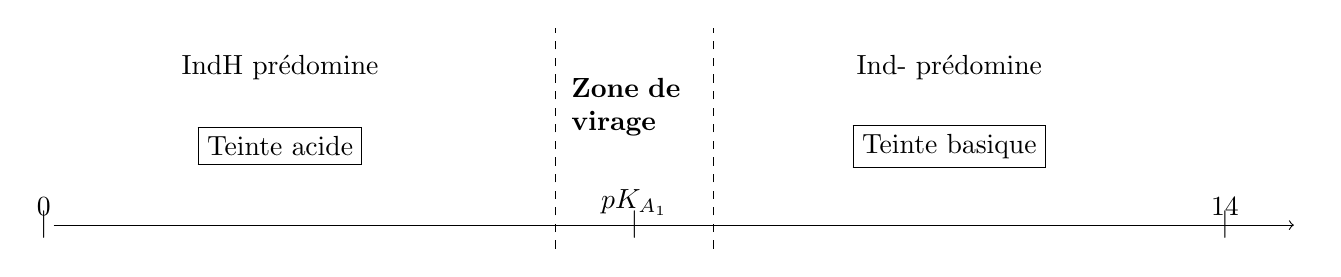
\begin{tikzpicture}
\node (O) at (0,0) {};
\node (A) at (7.5,0) {};
\node (C) at (15,0) {};
\node (F) at (16,0) {};
\draw (O) node{$|$} node[above]{0};
\draw (A) node{$|$} node[above]{$pK_{A_1}$};
\draw (C) node{$|$} node[above]{14};
\draw[->] (O) to (F);
\draw [dashed](6.5,-.3) -- (6.5,2.5);
\draw [dashed](8.5,-.3) -- (8.5,2.5);
\node (IndH) at (3,2) {\ce{IndH} prédomine};
\node (IndHT) at (3,1) {\fbox{Teinte acide}};
\node (Ind) at (11.5,2) {\ce{Ind-} prédomine};
\node (IndT) at (11.5,1) {\fbox{Teinte basique}};
\node [text width=2cm](ZV) at (7.7,1.5) {\textbf{Zone de virage}};
\end{tikzpicture}
\end{center}
Un indicateur coloré peut être utilisé pour \textbf{préparer l'équivalence d'un titrage} dont la réaction support est une réaction acide-base. Le \textbf{pH à l'équivalence} doit être compris dans la \textbf{zone de virage de l'indicateur} choisi.\\
\begin{minipage}{.5\textwidth}
\begin{center}
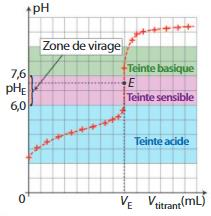
\includegraphics[scale=1]{Ressources/TSPE_C8_Cours_Fig2.png}
\end{center}
\end{minipage}\begin{minipage}{.5\textwidth}
\begin{tabular}{|>{\centering}m{2cm}|>{\centering}m{2cm}|>{\centering}m{2cm}|>{\centering\arraybackslash}m{2cm}|}
\hline \textbf{Nom} & \textbf{Teinte acide} & \textbf{Zone de virage} & \textbf{Teinte basique}\\
\hline Hélianthine & rouge & 3,1-4,4 & jaune\\
\hline Rouge de méthyle & rouge & 4,2-6,2 & jaune \\
\hline Bleu de bromothymol (BBT) & jaune & 6,0-7,6 & bleu\\
\hline Thymol-phtaléine & incolore & 9,3-10,5 & bleu\\
\hline 
\end{tabular}
\end{minipage}
\textbf{Exemple :} Lors du titrage ci-dessus, le pH à l’équivalence est proche de 7. Parmi les quatre indicateurs colorés proposés, seul le BBT convient car c’est le seul dont la zone de virage s’étend de part et d’autre du pH à l’équivalence (6,0 < $pH_E$ < 7,6).
\end{document}